%%%%%%%%%%%%%%%%%%%%%%%%%%%%%%%%%%%%%%%%%%%%%%%%%%%%%%%%
%   |------------------------------------------|       %
%   | Web App embebida en dispositivos móviles |       %
%   |  para la gestión de registros sobre la   |       %
%   |   contaminación de afluentes y ríos.     |       %
%   |                                          |       %
%   |          Proyecto de graduación          |       %
%   |__________________________________________|       %
%                                                      %
%   Autores                                            %
%   -------                                            %
%                                                      %
% * Bruno, Ricardo Hugo (CX 1409686)                   %
%     rburnount@gmail.com                              %
% * Gómez Véliz, Kevin Shionen (CX 1411828)            % 
%     ing.gomezvelizkevin@gmail.com                    %
%                                                      %
%   Tutor                                              %
%   -------                                            %
%                                                      %
% * Ing. Cohen, Daniel Eduardo                         %
%        dcohen.tuc@gmail.com                          %
%                                                      %
%   Cotutor                                            %
%   -------                                            %
%                                                      %
% * Ing. Nieto, Luis Eduardo                           %
%        lnieto@herrera.unt.edu.ar                     %
%                                                      %
%                                                      %
%%%%%%%%%%%%%%%%%%%%%%%%%%%%%%%%%%%%%%%%%%%%%%%%%%%%%%%%

\chapter{Disciplina de Requisitos}
\label{chap:requisito}

  \section{Introducción}

    Esta especificación tiene como objetivo analizar y documentar las necesidades funcionales que deberán ser soportadas por el sistema a desarrollar. Para ello, se identificarán los requisitos que ha de satisfacer el nuevo sistema mediante entrevistas, el estudio de los problemas de las unidades afectadas y sus necesidades actuales. Además de identificar los requisitos se deberán establecer las prioridades, las cuales proporcionan un punto de referencia para validar el sistema final, que comprueben que se ajusten a las necesidades del usuario.

  \section{Identificación de usuarios participantes}

    Los objetivos de esta tarea son identificar a los responsables de cada una de las unidades y a los principales usuarios implicados. Para ello se consideran los siguientes aspectos:

    \begin{itemize}
      \item Incorporación de usuarios al equipo de proyecto.
      \item Conocimiento de los usuarios de las funciones a automatizar.
      \item Repercusión del nuevo sistema sobre las actividades actuales de los usuarios.
      \item Implicaciones legales del nuevo sistema.
    \end{itemize}

      Se identificaron los siguientes usuarios:

    \begin{itemize}
      \item \emph{Grupo de Administradores:} Formado por los solicitantes del software en cuestión.
      
      \item \emph{Grupo de Alumnos:} Formado principalmente por alumnos de escuelas/colegios que realizan muestras, las cuales generan registros en el sistema.
    \end{itemize}

    Es de destacar la necesidad de una participación activa de los usuarios del futuro sistema en las actividades de desarrollo del mismo, con objeto de conseguir la máxima adecuación del sistema a sus necesidades y facilitar el conocimiento paulatino de dicho sistema, permitiendo una rápida implantación.

  \section{Educción de requisitos}

    \subsection{Estudio de Documentación. Planificación y Realización de Entrevistas}

      Esta tarea tiene como finalidad capturar los requisitos de usuarios para el desarrollo del sistema.

      Para el análisis de requisitos se usaron distintas técnicas de educción de requisitos. Entre ellas el estudio de la documentación provista por parte del administrador; entrevistas abiertas y estructuradas, análisis del proceso actual.

  \section{Especificación de Requisitos de Software}

    \renewcommand{\thesubsection}{\arabic{subsection}}
    \subsection{Introducción}

      Este documento es una Especificación de Requisitos Software de la  Web App embebida en dispositivos móviles para la gestión de registros sobre la contaminación de afluentes y ríos. Esta documentación es fruto de las entrevistas, estudio de la documentación y del funcionamiento del proceso actual, así como del análisis llevado a cabo por el equipo de desarrollo.

      El objetivo de la especificación es definir en forma clara, precisa, completa y verificable todas las funcionalidades y restricciones del sistema que se desea construir.

      Esta documentación está sujeta a revisiones por el grupo de administradores que se recogerán por medio de sucesivas versiones del documento, hasta alcanzar la aprobación por parte de los mismos. Una vez aprobado, servirá de base al equipo de desarrollo para la construcción del sistema en cuestión.

      Esta especificación se ha realizado de acuerdo al estándar “IEEE Recomended Practice for software Requirements Specifications(IEEE/ANSI 830-1993)”.


    \subsection{Objetivos y alcance del sistema}

      El presente proyecto tiene como objetivo principal ayudar al medio ambiente, utilizando un sistema de gestión que permite la creación y administración de registros, los cuales contienen datos de muestras del universo de estudio que, al ser procesadas, brinda el estado de contaminación de un río o afluente, mediante indicadores biológicos.
      Estos registros cuentan con contenido multimedia y coordenadas geográficas

  \section{Definiciones, acrónimos y abreviaturas}

    \subsection{Definiciones}
      \begin{itemize}
        
        \item \emph{Salida de campo:} La principal aportación de la salida de campo es que permite al alumnado adquirir un aprendizaje significativo en el que el principal elemento del proceso de enseñanza-aprendizaje es la construcción de significados. La persona aprende un concepto, un fenómeno, un procedimiento, un comportamiento, etc.
        
        \item \emph{Insectos:} Nuestro universo de estudio obliga solo a tener en cuenta 4 insectos, los cuales sirven para indicar el posible grado de contaminación del agua. Estos insectos son los siguientes:
        
        \begin{itemize}
          \item Elimidos.
          \item Patudos.
          \item Plecopteros.
          \item Tricopteros.
        \end{itemize}
        
        \item \emph{Muestra}: Una muestra esta compuesta por los insectos encontrados en una salida de campo. 
        
        \item \emph{Indice de Contaminación}: Para el sistema, el indice de contaminación es el valor calculado, mediante la cantidad de diferentes insectos encontrados en el universo de estudio, de la siguiente manera:
        
        \begin{table}[H]
          \centering
          \begin{tabular}{|p{3.8cm}|l|l|}
            \hline
            \centering
            Cantidad de insectos encontrados  & Indice & Interpretación \\ \hline 
            0                     & 0 & Muy contaminado \\ \hline
            1                     & 1 & Contaminado \\ \hline
            2                     & 2 & Con contaminación media \\ \hline
            3                     & 3 & En buen estado \\ \hline
            4                     & 4 & En excelente estado \\ 
            \hline
          \end{tabular}
        \end{table}
        
        \item \emph{Foto paisaje}: Foto obtenida del paisaje en donde se realizo la muestra de los insectos encontrados, con el fin de facilitar un punto de referencia visual para próximas salidas de campo.
        
        \item \emph{Foto insectos}: Foto obtenida de la muestra que sirve para que los administradores de la aplicación validen, o no, el registro en cuestión.
        
        \item \emph{Coordenadas geográficas}: Se usan para referenciar, mediante latitud y longitud, el lugar en donde se realizo el registro.
        
        \item \emph{Mapa}: Mapa digital (Google Maps) en donde se muestran los registros realizados por los usuarios.
        
        \item \emph{HTML:} HyperText Markup Language. Lenguaje de marcado para la elaboración de paginas web. En nuestro caso, genera la vista final del sistema.
        
        \item \emph{BD:} Base de datos.
        
        \item \emph{CRUD:} Es el acrónimo de ``Crear, Leer, Actualizar y Borrar'' (del original en ingles: Create, Read, Update and Delete), que se usa para referirse a las funciones básicas en bases de datos.
        
        \item \emph{MCVS:} Modelo de Ciclo de Vida del Sistema.
      \end{itemize}

  \section{Descripción general}

    Esta sección nos presenta una descripción general del sistema con el fin de conocer las funciones que debe soportar, los datos asociados, las restricciones impuestas y cualquier otro factor que pueda influir en la construcción del mismo.
    El sistema nace como necesidad de un grupo de docentes de la Facultad de Ciencias Naturales e Instituto Miguel Lillo, por llevar un control mas exhaustivo de su investigación.
    Es prioritario el seguimiento de la contaminación de los afluentes y ríos ubicados en la provincia de Tucumán.

    \subsection{Proceso actual}

      Este seguimiento se realizaba mediante salidas de campos con alumnos de las escuelas rurales donde realizaban las siguientes actividades:
      
      \begin{itemize}
        \item Los alumnos obtienen muestras del río o afluente intentando capturar algunos de los insectos del universo de estudio.
        
        \item Los docentes a cargo verifican dichas muestras, identificando las coincidencias, obteniendo de esta forma, un indice de contaminación.  
      \end{itemize}
      
      Todo esto se realiza de manera manual, anotando en papel y luego es transcripto a una planilla Excel.
      Todo el procedimiento antes descripto, dificulta la trazabilidad y administración de la información (introduciendo errores y demoras por el manejo manual de la información), por lo que todo esto sería más efectivo y sencillo con la ayuda de la tecnología. \newpage

    \subsection{Reingeniería de proceso}

      El objetivo de este proyecto se basa en proporcionar facilidades al proceso actual de la siguiente forma: 

      \begin{itemize}
        \item Dos imágenes capturadas con la cámara de fotos del Smartphone:
        
        \begin{itemize}
          \item La primera imagen será una foto de los insectos encontrados en un río o afluente. El objetivo es encontrar 4 insectos diferentes para analizar la biodiversidad.
         
          \item La segunda imagen será una foto del paisaje que servirá como un futuro punto de referencia para próximas salidas de campo. 
        \end{itemize}
        
        \item Capturar coordenadas de manera automática con una precisión propia al GPS integrado del Smartphone, las cuales se guardarán como \emph{latitud} y \emph{longitud}
        
        \item El usuario deberá seleccionar, según su criterio personal, cuales de los 4 insectos fueron encontrados por él, mediante un formulario interactivo, el cual consta de imágenes reales de los mismos para una buena comparación y un campo de observaciones para realizar comentarios subjetivos sobre la muestra en cuestión.
        
        \item Al completar toda la información mencionada anteriormente, se visualizará una ruleta virtual animada, la cual mostrará un valor (indice de contaminación), indicando el posible grado contaminación del agua en donde se realizo la muestra.

        \item Lo anterior se realizará sin conexión a internet (2G, 3G, Wifi, etc), generando un registro de manera local, que luego, de manera automática, se subirá a los servidores al momento de adquirir alguna conexión a internet.

        \item Los administradores podrán gestionar, mediante un navegador web (Google Chrome, Internet Explorer, Mozilla, etc) o desde la aplicación en el Smartphone, los registros previamente creados y guardados en el servidor.

        \item Analizando todos los registros, se creará un renderizado de un mapa  (Google Maps) en donde los administradores y usuarios podrán visualizar, con trazos de diferentes colores, el grado de contaminación del agua en el curso de los ríos o afluentes analizados en las salidas de campo.
      \end{itemize}

      El sistema debe ser seguro, escalable, de fácil mantenimiento y muy simple de usar utilizando solo interfaces táctiles para los usuarios finales. El futuro sistema llevará el nombre \emph{Agüita}.

      Las funciones que debe realizar el sistema se pueden agrupar de la siguiente manera:

      \begin{itemize}

        \item \emph{Gestión de usuarios:} Debe permitir gestionar los usuarios (CRUD). Los mismos pueden ser usuarios o administradores del sistema.
        Para que un usuario pueda generar un registro, deberá estar previamente registrado e iniciar sesión por una única vez en su Smartphone.
        Los usuarios deben poder configurar/modificar las opciones de su perfil como ser: nombre, apellido, lugar de residencia, institución a la que pertenece y grado correspondiente.
        Los usuarios no pueden consultar la información personal de otros usuarios.

        \item \emph{Gestión de registros:} Debe permitir gestionar los registros (CRUD). Los usuarios generar registros. Los administradores pueden interactuar con los mismos, cambiando su estado (pendiente - valido - invalido) según la información brindada por los mismos (no verificada por los administradores - correcta - incorrecta) respectivamente.

        \item \emph{Consultas de registros realizados:} Los usuarios podrán consultar un listado de sus registros creados con la información completa.
        Los usuarios no podrán consultar los registros de otros usuarios.
        Los administradores podrán ver los registros creados por los todos los usuarios de la aplicación con toda su información correspondiente.

        \item \emph{Consulta de mapa:} Los usuarios y administradores pueden ver el mapa final con toda la información recopilada de todos los registros creados por los mismos.
        Todos los registros que estén en un estado \emph{rechazado} no se eliminaran de la base de datos, no obstante, los mismos no se tomaran en cuenta para el renderizado del mapa final. 

      \end{itemize}
      \newpage 
  \section{Requisitos específicos}

    \begin{enumerate}[A.]
      \item \textbf{Gestión de Usuarios}
        \begin{itemize}  
          \item \textbf{Alta de usuarios:}
            \\ \textbf{Introducción:} El sistema permite introducir información sobre usuarios en la aplicación.
            \\ \textbf{Entrada:} IdUsuario + Email + Usuario + Contraseña + Nombre + Apellido + Institución + Grado + Residencia + Rol + Foto Perfil + Estado 
            \\ \textbf{Proceso:} El sistema comprueba la inexistencia previa de un usuario, buscando coincidencias en el nombre de usuario y mail. En caso de no encontrar un usuario con los nombre de usuario y mail especificados, se creará y guardará el nuevo usuario, al cual se le asignará el número único IdUsuario (este número se obtiene a partir del máximo existente hasta el momento, siendo 1 para el primer usuario). En este caso, se devolverá un mensaje de éxito y el IdUsuario. En caso que ya existiera un usuario con los nombre de usuario y mail especificados, se devolverá un mensaje de error informando tal situación
            \\ \textbf{Salida:} @IdUsuario + mensaje
            \\
          \item \textbf{Modificación de usuarios:}
            \\ \textbf{Introducción:} El sistema permite modificar información sobre usuarios existentes en la aplicación.
            \\ \textbf{Entrada:} @IdUsuario + Nombre + Apellido + Institución + Grado + Residencia + Foto Perfil
            \\ \textbf{Proceso:} El sistema comprueba la existencia previa de un usuario en base a @IdUsuario y actualiza la información del mismo. En caso de éxito, se devolverá un mensaje de éxito y el IdUsuario. En caso de error se devolverá un mensaje con el motivo del mismo.
            \\ \textbf{Salida:} @IdUsuario + mensaje
            \\
          \item \textbf{Cambiar estado de usuarios:}
            \\ \textbf{Introducción:} El sistema permite habilitar/inhabilitar usuarios existentes en la aplicación.
            \\ \textbf{Entrada:} @IdUsuario + Estado Actual
            \\ \textbf{Proceso:} El sistema comprueba la existencia previa de un usuario en base a @IdUsuario para poder modificar su estado. Hay dos tipos de estado: ``Habilitado'' - ``Inhabilitado''. Este proceso permuta el estado actual del usuario. Si un usuario tiene estado ``Habilitado'', este se cambia a ``Inhabilitado'' y viceversa. Los registros asociados al usuario no deben eliminarse ni modificarse. En caso de error se devolverá un mensaje con el motivo del mismo.
            \\ \textbf{Salida:} @IdUsuario + Mensaje
            \\
          \item \textbf{Ver detalles de usuario:}
            \\ \textbf{Introducción:} El sistema permite ver detalles relacionados a los usuarios existentes en él. Se debe visualizar usuario, nombre, apellido, institución, grado, residencia, foto de perfil y cantidad de registros generados
            \\ \textbf{Entrada:} @IdUsuario
            \\ \textbf{Proceso:} El sistema comprueba la existencia previa del usuario en base a @IdUsuario. En caso de éxito, se presenta la información del mismo. En caso de error se devolverá un mensaje con el motivo del mismo.
            \\ \textbf{Salida:} Usuario + Nombre + Apellido + Institución + Grado + Residencia + Email + Foto Perfil + Cantidad Registros
            \\
          \item \textbf{Cambiar contraseña de usuario:}
            \\ \textbf{Introducción:} El sistema permite cambiar la contraseña a los usuarios existentes en él.
            \\ \textbf{Entrada:} @IdUsuario + Contraseña Anterior + Contraseña Nueva
            \\ \textbf{Proceso:} El sistema comprueba la existencia previa del usuario en base a @IdUsuario, luego se impactara la nueva contraseña, dejando en desuso la anterior. En caso de éxito, se presenta la información del mismo. En caso de error se devolverá un mensaje con el motivo del mismo.
            \\ \textbf{Salida:} @IdUsuario + Mensaje
            \\
          \item \textbf{Cambiar rol de usuario:}
            \\ \textbf{Introducción:} El sistema permite cambiar el Rol a los usuarios existentes en él. Esta acción solo la pueden realizar los usuarios del grupo ``Administradores''
            \\ \textbf{Entrada:} @IdUsuario + Rol
            \\ \textbf{Proceso:} El sistema comprueba la existencia previa del usuario en base a @IdUsuario. Hay dos tipos de roles: ``Administrador'' - ``Usuario''. Este proceso modificará el Rol del mismo según valor de entrada. En caso de éxito, se presenta la información del mismo. En caso de error se devolverá un mensaje con el motivo del mismo.
            \\ \textbf{Salida:} @IdUsuario + Mensaje
            \\
          \item \textbf{Búsqueda de usuarios:}
            \\ \textbf{Introducción:} El sistema permite introducir parámetros con los que se buscará usuarios que coincidan con los mismos.
            \\ \textbf{Entrada:} Usuario o Nombre o Apellido o Email
            \\ \textbf{Proceso:} El sistema lista al usuario que cumpla con los parámetros de búsqueda en caso de coincidencia. En caso de no encontrar algún usuario, se mostrará un mensaje vacío, indicando que la búsqueda no arrojo resultados.
            \\ \textbf{Salida:} Usuario + Nombre + Apellido + Institución + Grado + Residencia + Email + Foto Perfil + Cantidad Registros
            \\
        \end{itemize}

      \item \textbf{Gestión de Registros}
        \begin{itemize}
          \item \textbf{Alta de registros:}
            \\ \textbf{Introducción:} El sistema permite dar de alta un nuevo registro ingresando indice, insectos encontrados, fecha, latitud, longitud, foto del paisaje, foto de la muestra, foto del mapa (vista aérea con un PIN indicando la ubicación terrestre), observaciones del usuario, IdUsuario (creador del registro), IdUbicacion (país, localidad, provincia).
            \\ \textbf{Entrada:} IdRegistro + Indice + Insectos Encontrados + Fecha Creación + Latitud + Longitud + Foto Paisaje + Foto Muestra + Foto Mapa + Observaciones Usuario + IdUsuario + IdUbicación
            \\ \textbf{Proceso:} El sistema crea un registro al cual se le asignará el número único IdRegistro (este número se obtiene a partir del máximo existente hasta el momento, siendo 1 para el primer registro). Los estados de validación posibles son ``Valido'', ``Invalido'' y ``Pendiente''. Un registro nuevo se creará con un valor de estado de validación igual a ``Pendiente''.  y con observaciones del administrador sin contenido, además, las fotos se almacenarán en Base64. En caso de éxito, se devolverá un mensaje de éxito y el IdRegistro.
            \\ \textbf{Salida:} IdRegistro + Mensaje
            \\
          \item \textbf{Cambiar estado de registros:}
            \\ \textbf{Introducción:} El sistema permite cambiar el estado de un registro. Solo los administradores del sistema tendrán los permisos para realizar esta acción. Se podrá cambiar el estado del registro ``Valido'' / ``Invalido'' y viceversa. Inicialmente, el registro se crea con un estado ``Pendiente'', el cual, una vez modificado, no se podrá volver a asignar.
            \\ \textbf{Entrada:} @IdRegistro + Estado Validación
            \\ \textbf{Proceso:} El sistema modifica el registro con el valor de estado validación correspondiente. En caso de éxito, se devolverá un mensaje de éxito y el IdRegistro.
            \\ \textbf{Salida:} IdRegistro + Mensaje
            \\
          \item \textbf{Asignar observaciones de administrador a registros:}
            \\ \textbf{Introducción:} El sistema permite agregar observaciones de administrador al registro. Solo los administradores del sistema tendrán los permisos para realizar esta acción.
            \\ \textbf{Entrada:} @IdRegistro + Observaciones Administrador
            \\ \textbf{Proceso:} El sistema modifica el registro agregando una observación de administrador. En caso de éxito, se devolverá un mensaje de éxito y el IdRegistro.
            \\ \textbf{Salida:} IdRegistro + Mensaje
            \\
          \item \textbf{Ver detalles de registro:}
            \\ \textbf{Introducción:} El sistema permite ver detalles relacionados a los registros existentes en él. Se debe visualizar indice, insectos encontrados, fecha, latitud, longitud, foto del paisaje, foto de la muestra, foto del mapa, observaciones del usuario, estado de validación, usuario que lo creó, país, provincia, localidad.
            \\ \textbf{Entrada:} @IdRegistro
            \\ \textbf{Proceso:} El sistema comprueba la existencia previa del registro en base a @IdRegistro. En caso de éxito, se presenta la información del mismo. En caso de error se devolverá un mensaje con el motivo del mismo.
            \\ \textbf{Salida:} Indice + Insectos Encontrados + Fecha Creación + Latitud + Longitud + Foto Paisaje + Foto Muestra + Foto Mapa + Observaciones Usuario + Observaciones Administrador + Estado Validación + IdUsuario + IdUbicación
            \\
          \item \textbf{Búsqueda de registros}
            \\ \textbf{Introducción:} El sistema permite buscar registros filtrando por los registros creados desde un intervalo de fechas, por estado de validación, por indice.
            \\ \textbf{Entrada:} Fecha Inicio Fecha Fin + Estado Validación + Indice
            \\ \textbf{Proceso:} El sistema lista los registros que cumplan con los parámetros de búsqueda en caso de coincidencia. En caso de no encontrar algún registro, se mostrará un mensaje vacío, indicando que la búsqueda no arrojo resultados. Si la búsqueda no contiene parámetros, se listan todos los registros existentes en el sistema
            \\ \textbf{Salida:} Indice + Insectos Encontrados + Fecha Creación + Latitud + Longitud + Observaciones Usuario + Observaciones Administrador + Estado Validación + IdUsuario + IdUbicación
        \end{itemize}

      \item \textbf{Gestión de Mapas}
        \begin{itemize}
          \item \textbf{Ver mapa}
          \\ \textbf{Introducción:} El sistema permite ver el mapa interactivo con la información de los registros almacenados que cumplan con la condición de estado de validación igual a ``Valido''.
          \\ \textbf{Entrada:} Arreglo de Registros 
          \\ \textbf{Proceso:} Mostrar un mapa con puntos obtenidos mediante la latitud y longitud de cada registros del arreglo.
          Los puntos indican, ademas de la posición geográfica del registro, el usuario que lo creó y el indice de contaminación numéricamente y ademas con un color de entre 4 diferentes para una rápida identificación visual.
          \\ \textbf{Salida:} Mapa + Puntos Geográficos
        \end{itemize}

    \end{enumerate}

    \subsection{Suposiciones y Dependencias}
      \begin{itemize}
        \item \textbf{Suposiciones:} Se asume que los requisitos en este documento son estables una vez que sean aprobados por los responsables de la aplicación. Cualquier petición de cambios en la especificación debe ser aprobada por todas las partes intervinientes y será gestionada por el equipo de desarrollo.
        \item \textbf{Dependencias:} El sistema trabaja en conjunto con Google Maps y el sistema de posicionamiento global mediante satélites, algún cambio que se realicen en estos, el sistema podría presentar inconsistencias, errores, y hasta dejar de funcionar.
      \end{itemize}

    \subsection{Requisitos de Usuario y Tecnológicos}
      \begin{itemize}
        \item \textbf{Requisitos de usuario:} Como se mencionó anteriormente, se identifican dos tipos de usuarios: Administradores y Alumnos. Los usuarios tendrán sus cuentas asociadas con Nombre de Usuario y Contraseña. Los mismos podrán iniciar sesión desde computadoras de escritorio (Sistema de administración y gestión de registros) o mediante la aplicación para dispositivos móviles Smartphones, siempre y cuando, dispongan de una cuenta valida. En caso contrario, deberán registrarse en el sistema mediante la aplicación correspondiente.

        \item \textbf{Requisitos tecnológicos:} Los administradores podrán iniciar sesión en el sistema mediante computadoras de escritorio, facilitando la gestión y administración del mismo. Ésta versión WEB restringe el uso a aquellos usuarios del grupo ``Alumnos'', por otra parte, los alumnos podrán hacer uso del sistema solo para generar registros, y ver el mapa interactivo mediante la aplicación para Smartphones que deberán descargar la tienda.
        Se utilizará una plataforma de servicios en la nube o un servidor físico local provisto por el cliente de este sistema, para administrar una máquina virtual que hará de servidor web y servidor de base de datos. El sistema operativo que correrá la máquina virtual será Ubuntu Server, éste es un sistema operativo gratuito y de código abierto, por otra parte, el sistema gestor de base de datos será del tipo MySQL. Ambos sistemas (operativo y gestor de base de datos), serán instalados en su ultima versión estable al momento de la entrega del software.
        El sistema se ejecutara sobre un esquema de peticiones Cliente/Servidor (API Rest). La elección esta infraestructura se debe principalmente a 3 motivos: 
        \begin{itemize}
          \item Debido a que el sistema se puede usar mediante Smartphones y computadoras de escritorio de forma remota, la solución fue dividir y separar, como ya se menciono, la aplicación para los usuarios de el servidor de consultas y base de datos.
          \item Experiencia del equipo de desarrollo 
          \item Sistemas seleccionados de licencia gratuita.
        \end{itemize}
      \end{itemize}

    \subsection{Requisitos de Interfaces Externas}
      \begin{itemize}
        \item \textbf{Interfaz de usuario:} Las interfaces de la aplicación deben ser intuitivas, fáciles de usar, amigables y de respuesta rápida. La interfaz de usuario debe ser orientada al uso táctil de los Smartphones.
        \item \textbf{Interfaz Hardware:} 
          \begin{itemize}
            \item Requisitos para los Smartphones:
              \begin{itemize}
                \item Los Smartphones de los usuarios que ejecutaran la aplicación deberán tener las siguientes características independientemente de su S.O:
                  \begin{itemize}
                    \item Cámara fotográfica de 1 Mega Pixeles o más.
                    \item GPS integrado.
                    \item Conexión a internet vía WiFi o Red GSM
                    \item Pantalla táctil de 3.5'' o superior.
                    \item Espacio disponible de 10 MB para la instalación de la aplicación + Cantidad de MB variable ocupado por cada registro creado. 
                  \end{itemize}
              \end{itemize}
            \item Requisitos mínimos para el servidor:
            \begin{itemize}
              \item Procesador AMD Sempron 3000 o equivalente o procesador Intel Celeron o equivalente. Capacidad de virtualización
              \item 1 GB de memoria RAM.
              \item Conexión a internet.
            \end{itemize}
            \item Requisitos mínimos para las PC o notebook de los administradores
            \begin{itemize}
              \item Procesador AMD Sempron 3000 o equivalente. Procesador Intel Celeron o equivalente.
              \item 1 GB de memoria RAM.
              \item Periféricos de entrada/salida.
              \item Conexión a internet
            \end{itemize}
          \end{itemize}
      
        \item \textbf{Interfaz Software:} 
          Sistemas operativos soportados por la aplicación:
          \begin{itemize}
            \item Smartphones 
            \begin{itemize}
              \item Android 4.0 o posterior.
              \item iOS 9.0 o posterior.
            \end{itemize}
            \item Servidor 
            \begin{itemize}
              \item  El sistema operativo será Ubuntu Server en su ultima versión estable LTS. 
            \end{itemize}
            \item PC o notebook de los administradores 
            \begin{itemize}
              \item Cualquier sistema operativo con navegador web 
            \end{itemize} 
          \end{itemize}
      \end{itemize}

    \subsection{Requisitos de Rendimiento}

      El Tiempo de respuesta de la aplicación de cada función solicitada por el usuario no debe ser superior a los 3 segundos en una velocidad efectiva de conexión con el servidor a través de 3G.
      No obstante, los registros al generarse de manera offline (sin conexión a internet), se guardarán de manera local, por lo que si se generaron varios registros, al momento de que el Smartphone detecte conexión a internet, el tiempo de respuesta se ve afectado de manera directamente proporcional a la cantidad de registros que se estén subiendo al servidor en la nube en ese momento.

    \subsection{Requisitos de Desarrollo y Restricciones de Diseño}

      El ciclo de vida será Prototipado Evolutivo, debiendo orientarse hacia el desarrollo de un sistema flexible que permita incorporar de manera sencilla cambios y nuevas funcionalidades.

    \subsection{Ajuste a estándares} Interfaz de usuario basada Material Desing (Google)

    \subsection{Seguridad} 
      \begin{itemize}
        
        \item \textbf{En desarrollo:} Los desarrolladores acceden a la gestión del sistema operativo y/o sus aplicaciones a través de Secure Shell o SSH, el estándar de facto para la administración remota de servidores de manera segura. Tanto para la administración propia del servidor, como en las aplicaciones que se utilizan para administrar la base de datos (MySQL Workbench) y la gestión de archivos (SFTP), se realizan con clientes que establecen conexiones seguras con el servidor. La técnica empleada para dichas conexiones es el intercambio de claves públicas y validación con la clave privada de las aplicaciones cliente.
        \item \textbf{En producción:} Los usuarios del sistema acceden al mismo mediante la aplicación móvil o cualquier explorador web. Para operar con la aplicación, deben proveer un usuario y una contraseña. Esta información es procesada en el servidor en un proceso de validación de credenciales y devuelve al cliente el mensaje de inicio de sesión correcto. La comunicación entre cliente servidor viajara encriptada mediante el protocolo \gls{HTTPS}.
        \item \textbf{Roles y permisos:} Para reforzar la seguridad de la aplicación, cada usuario posee un rol (``Administrador'' o ``Alumno''), el cual tiene asociados diferentes permisos. Esto permite restringir el acceso a usuarios del grupo ``Alumno'' a la aplicación WEB de gestión y administración de registros. El rol ``Administrador'' tiene todos los permisos y privilegios, pudiendo así, gestionar el sistema e incluso generar registros como lo harían los Alumnos.
        \item \textbf{Red:} En la capa de red se crearon reglas de acceso al servidor mediante el uso del firewall provisto por el Sistema Operativo Ubuntu. A través de estas reglas se establece que servicios podrá ofrecer el servidor a los clientes de la aplicación.
        \item \textbf{Sistema Operativo:} En el sistema operativo se definen los usuarios y los permisos que poseen para realizar lecturas, escrituras y/o ejecuciones de archivos alojados en la memoria del servidor. De esta forma se previene que usuarios no autorizados puedan modificar, eliminar y ejecutar archivos en el servidor, incluso en la base de datos.
        \item \textbf{Servidor web:} A nivel servidor web, se prevé la implementación del protocolo de aplicación HTTPS que permite encriptar el trafico de información desde el servidor web hacia los navegadores o aplicaciones que realicen solicitudes, estableciendo un eslabón mas en la seguridad del sistema.
        \item \textbf{Política de respaldo:} El administrador llevará a cabo un respaldo de datos en discos externos o en la nube por el tiempo que el considere necesario. Ademas, se exportaran los registros en un archivo excel manteniendo la información necesaria para la recuperación de los registros a futuro.
        Por otro lado, el motor de Base de datos estará configurado para realizar backups cada cierto intervalo de tiempo definido por el administrador. Conservar los respectivos archivos de respaldo de los últimos 6 backups.
        \item \textbf{Política de Borrado:} No se ha definido
      \end{itemize}
      
  \section{Estimación del proyecto}

    \subsection{Planificación de etapas} 
      \begin{table}[H]
        \centering
        \begin{tabular}{|l|l|l|l|}
          \hline
          \centering
          Código  & Descripción  & Fecha Inicio & Fecha Fin \\ \hline
          A       & Estudio de factibilidad y acciones preliminares & 15/01/2017 & 25/01/2017 \\ \hline
          B       & Educción de requisitos & 01/02/2017 & 01/03/2017 \\ \hline
          C       & Diseño del prototipo & 02/03/2017 & 01/04/2017 \\ \hline
          D       & Corroborar diseño con requisitos & 01/04/2017 & 05/04/2017 \\ \hline
          E       & Desarrollo del prototipo & 10/04/2017 & 15/09/2017\\ \hline
          F       & Pruebas del prototipo & 15/09/2017 & 15/10/2017 \\ \hline
          G       & Refinamiento del prototipo & 15/11/2017 & 01/02/2018 \\ \hline
          H       & Análisis y evaluación el prototipo por parte del cliente & 15/02/2018 & 16/02/2018 \\ \hline
          I       & Refinamiento del prototipo & 01/03/2018 & 01/06/2018 \\ \hline
          J       & Entrega para producción & 15/09/2018 & 20/09/2018 \\ \hline
          K       & Seguimiento del sistema & 20/09/2018 & - \\ \hline
        \end{tabular}
        \caption {Fechas tentativas por etapa.}
      \end{table}

    \subsection{Duración estimada de tareas} 
      \begin{table}[H]
        \centering
        \begin{tabular}{|l|l|l|}
          \hline
          \centering
          Etapas  & Semanas  & Valor \% \\ \hline
          Estudio de factibilidad y acciones preliminares & 6 & 9\% \\ \hline
          Educcion de requisitos & 4 & 6\% \\ \hline
          Diseño del prototipo & 5 & 8\% \\ \hline
          Corroborar diseño con requisitos & 1 & 1\% \\ \hline
          Desarrollo del prototipo & 21 & 33\% \\ \hline
          Pruebas del prototipo & 4 & 6\% \\ \hline
          Refinamiento del prototipo & 11 & 17\% \\ \hline
          Análisis y evaluación el prototipo por parte del cliente & 1 & 1\% \\ \hline
          Refinamiento del prototipo & 12 & 18\% \\ \hline
          Entrega para producción & 1 & 1\% \\ \hline
          Seguimiento del sistema & - & - \\ \hline
          \textbf{Total} & 66 & 100\% \\ \hline
        \end{tabular}
        \caption {Estimación en semanas - Valor porcentual}
      \end{table}

    \subsection{Diagrama de Gantt} 

    \begin{figure}[htbp]
      \centering
        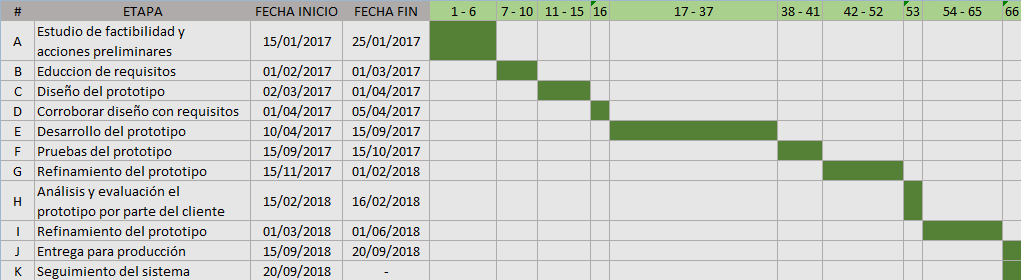
\includegraphics[width=1\textwidth]{imagenes/gantt.png}
    \end{figure} 